% Chapter Template

\chapter{Conclusions} % Main chapter title

\label{Chapter6} % Change X to a consecutive number; for referencing this chapter elsewhere, use \ref{ChapterX}

\lhead{Chapter 6. \emph{Conclusions}} % Change X to a consecutive number; this is for the header on each page - perhaps a shortened title

%----------------------------------------------------------------------------------------
%	SECTION 1
%----------------------------------------------------------------------------------------

\section{Conclusions}
This report has covered the general motivations of SUSY. One particular search, $\alpha_T$ has been described and its effectiveness after turn-on has been explained. The results from searches such as $\alpha_T$ are presented using simplified models allowing their reach in parameter space to be quantified. While this has deeply constrained new theories of physics the central motivation for low mass SUSY -- to stabilise the Higgs mass naturally -- remains. The LHC upgrade will provide significantly increased energies and luminosities. The effect this will have on SUSY production cross sections is shown in figure \ref{snow}\cite{ProjectedCx}. As can be seen the quantity of predicted SUSY events will be significantly increased. If low mass SUSY is physical then the LHC upgrade and $\alpha_T$ will provide an excellent opportunity for discovery. 
\begin{figure}
\centering
    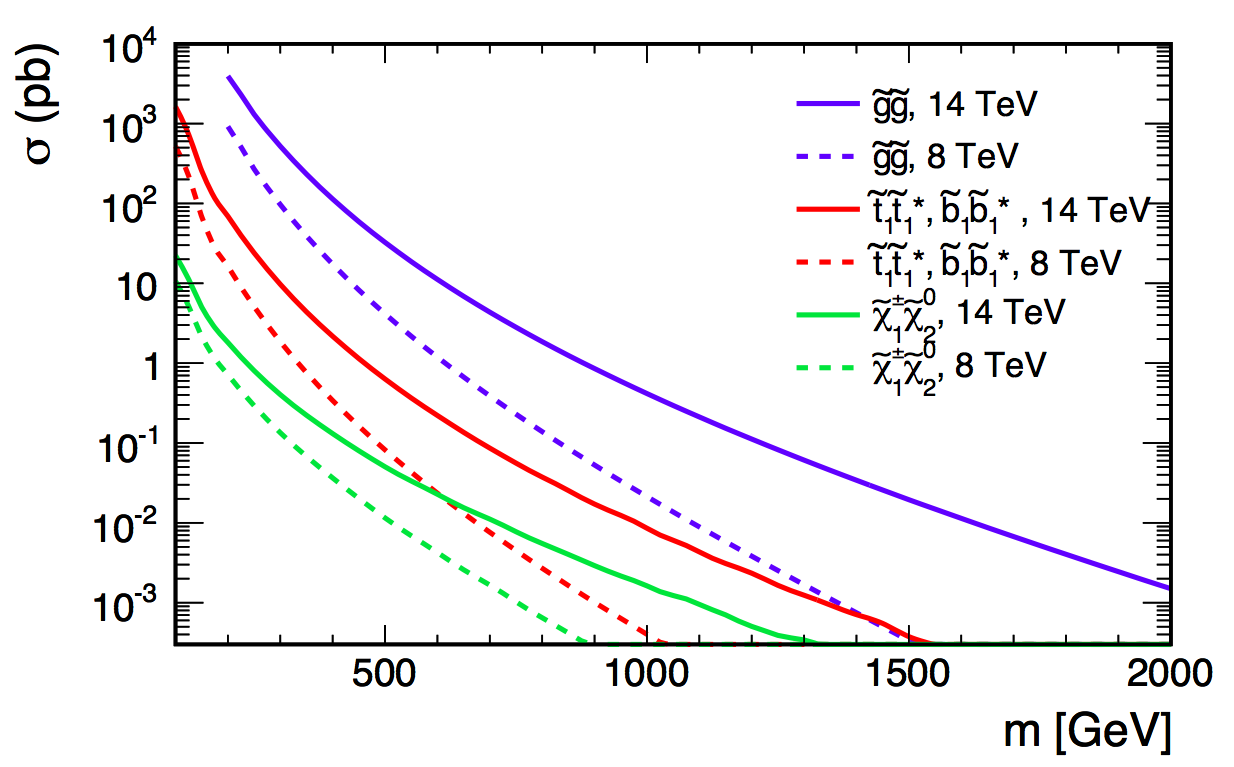
\includegraphics[width=0.8\textwidth]{Figures/snowmass.png}
  \caption{SUSY production cross sections at 14 TeV compared with 8TeV}
  \label{snow}
\end{figure}


